\chapter{Evaluation \& Testing}
\label{ch:Evaluation}


\section{Testing Methodology}

The testing programme was structured around two guiding principles. First, the evaluation of the supervised XGBoost regression model was conducted on data withheld from the fitting process, ensuring that reported performance figures reflect generalisation capability rather than  memorisation of training the training samples. Second, the explanation layer requires an independent testing discipline, since the correctness of its output cannot be inferred from the predictive accuracy of the underlying SHAP model alone. 

Four categories of tests were conducted: quantitative performance evaluation of the predictive model against a held-out test partition; behavioural testing of the explanation layer through additivity, consistency, and directional credibility cheques; integration testing of the end-to-end prediction pipeline via the FastAPI endpoints; and usability evaluation conducted with 
prospective end-users.

Beyond quantitative and behavioural testing, the fully integrated application was evaluated through structured user testing sessions, reflecting the project objective of assessing how end-users perceive and interact with the final deliverable. Participants were presented with the complete system that encompasses price prediction, SHAP-based feature attribution, and the frontend interface  and asked to complete a series of predefined scenarios representative of realistic usage. Feedback was collected following each scenario to capture both task performance and subjective user perception, including the interpretability of the model's explanations and the overall usability of the interface.


\section{Predictive Performance}

The cleaned and encoded dataset was partitioned into a 80\% training set and a 20\% evaluation set using the \verb|scikit-learn| \verb|train_test_split()| function.

The model achieved a Coefficient of Determination ($R^2$) of 0.9557 in the held-out partition, indicating that the fitted estimator accounts for approximately 95.57\% of the variance in the log-transformed price variable across unseen listings.

To complement the statistic $R^2$, the Mean Absolute Error (MAE) was calculated in the logarithmic transformed target space and subsequently inverted to the pound-sterling scale, producing a value of \pounds56,451. Given that the training data include high-value residential properties, this margin represents a reasonable absolute error relative to the typical price range of the considered listings.

\subsection{Limitations and Transparency}

Although the model achieves a strong $R^2$ of $0.9557$ and an MAE of \pounds56,451, it is important to recognise that the predictions carry inherent uncertainty and should not be treated as definitive valuations. The training dataset comprises 977 properties scraped from Zoopla, which introduces selection bias; the model reflects the distribution of listings available at the time of scraping rather than the full breadth of the UK property market. 

Features such as neighbourhood desirability, property condition, and recent local market shifts are not captured in the dataset, meaning that the model can systematically predict certain properties with inaccuracy. To mitigate the risk of misleading users, PropertyIQ presents ML predictions alongside the asking price and SHAP-derived feature explanations, making the reasoning behind each estimate transparent and auditable. Users are implicitly \textbf{discouraged from treating the predicted value as a ground truth and instead are guided to use it as one data point within a broader investment decision-making process}.


\section{SHAP Explanation Layer Review}

The explanation layer was evaluated against three properties whose correctness the broader system depends upon and which cannot be derived from predictive performance alone. The additivity was verified by confirming that the aggregated SHAP values were aligned, with numerical precision, with the difference between the model output and the expected base value; a result that is theoretically guaranteed by \verb|TreeExplainer|, which computes exact Shapley values rather than sampling-based approximations. 

Consistency was established by confirming that repeated calls to \verb|predict_and_explain| with identical inputs produced exactly identical decompositions in all iterations. Although directional credibility was assessed through controlled feature perturbations: increasing gross internal floor area produced positive SHAP contributions; reducing years remaining on a leasehold below standard 
thresholds produced negative contributions; and substituting the postcode sector between central London and regional identifiers produced the expected shift in locational attribution. 

In each case, the observed behaviour was consistent with the hedonic pricing relationships discussed in Section \ref{ch:Background} \nameref{ch:Background}.


\section{User Testing}

To complement the quantitative and behavioural evaluation reported in the following subsections, a \textbf{user testing exercise was conducted to gather qualitative feedback on how the project pipeline presents itself to potential users} of the PropertyIQ web application, in Figure \ref{fig:webapp}.

\begin{figure}[h]
    \centering
    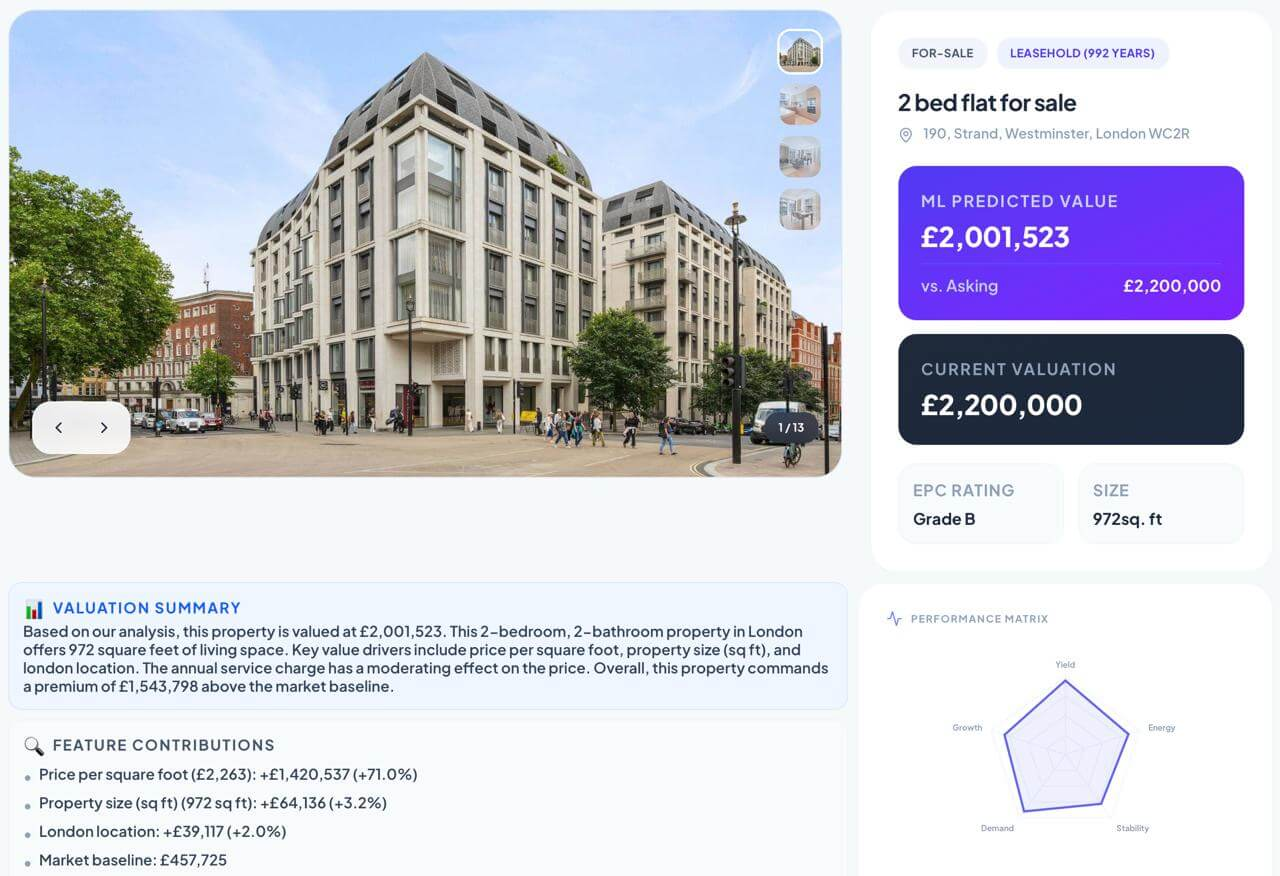
\includegraphics[width=\textwidth]{eval/images/webapp.jpeg}
    \caption{PropertyIQ webapp with predicted value and explanation.}
    \label{fig:webapp}
\end{figure}


\subsection{Small-scale individual property investor}
\label{su:SmallScaleInvestor}

The first participant was a small-scale individual investor who had a modest residential portfolio with no prior exposure to explainability-based tools of the kind developed in this project. Their response was informed by the contrast between the platform and their current practice, which requires them to perform due diligence on each property manually to assess whether the asking price represents fair value. 

The prospect of obtaining a decomposed valuation at the click of a button, in place of a process they estimated at approximately two hours of work per property, was described as a substantial improvement on their current workflow and constitutes one of the clearest articulations of the efficiency gain the pipeline is capable of delivering for individual investors.

The participant also responded with notable enthusiasm to the risk early warning component, which is identified in Section \ref{se:FutureWork} \nameref{se:FutureWork}. They explained that as holders of illiquid residential assets, they have no continuous means of evaluating the condition or current value of their holdings and must engage a professional surveyor at a significant cost whenever such an assessment becomes material. 

In their view, a platform capable of surfacing risk indicators against properties already owned was a natural and commercially valuable extension of the core valuation tool. Their feedback also included a concrete feature suggestion, namely a side-by-side comparison mode in which two properties could be evaluated against each other, and a recommendation surfaced as to which represented the strongest proposition, a suggestion that aligns with the tradition of comparative assessment described in Section \ref{se:GeneralBenfits} \nameref{se:GeneralBenfits}.

The only reservation offered concerned the depth of the explanation layer itself, with the participant indicating that a more detailed accompanying text would further improve the interpretability of individual feature contributions. However, in general, the session was markedly positive, and the participant expressed confidence in the near-term prospects of such a platform.


\subsection{Prospective first-time buyer}

The second participant was actively considering their first residential purchase and had no previous exposure to such tools. Once the conceptual basis of the platform was explained, a predictive valuation was paired with a feature-level account of how that valuation was generated. 

Their response was enthusiastic, and the reasoning they offered for that enthusiasm merits recording in some detail, as it speaks directly to user-trust motivations. They described the difficulty of evaluating individual properties without a reliable reference point and reported a repeating experience in which selling agents, when pressed on the basis of an asking price, deflected the question on the grounds that they were only representing the seller's stated figure rather than justifying it. 

The prospect of a tool capable of decomposing a valuation into its constituent drivers was, in their words, materially useful to someone preparing to make their first purchase.
The feedback, following the interactive session, was consistent with the initial reaction. The participant engaged positively with the SHAP-generated explanation layer, describing it as the element that distinguished the platform from the conventional listing-based tools they had previously encountered. 

The simplified interface and general visual presentation of the application were each praised, and the participant made repeated use of the prediction functionality against the set of integrated properties to develop a better understanding of how the contributions of features shifted across comparable listings. Their principal reservation, offered as a constructive feature, concerned the depth of the natural-language explanation itself: while the concept and its execution were well received, the participant expressed a preference for longer and more granular explanatory text, particularly for features they did not immediately recognise.


\section{Evaluation}

The testing demonstrated that PropertyIQ met most of the objectives set in Appendix \ref{ch:Specifications} \nameref{ch:Specifications}. The predictive ML model performs at a level broadly consistent with the benchmarks reported for tree-based ensemble methods in the property valuation literature \parencite{Ho2020} \parencite{Rico-Juan2021}.
The explanation layer produces attributions that are mathematically accurate, reproducible on repeated calls, and directionally consistent with the hedonic pricing relationships. In general, these outcomes support the view that the system occupies a credible middle ground between predictive accuracy and interpretability, which the literature review identified as the central trade-off confronting ML evaluation tools.

Integration testing against the FastAPI endpoints confirmed that the valuation and explanation pipelines behaved consistently when invoked through the same interface used by the frontend. This distinction is significant because the preprocessing logic that reconstructs the feature vector at inference time introduces a class of errors that would remain hidden during offline evaluation. 

No discrepancies were observed between notebook and endpoint-based predictions on matched inputs, suggesting that the separation between training artefacts and deployed application was implemented with sufficient precision to preserve the integrity of the attribution results.

Although limited in scale, the usability sessions served as a corrective to the assumption that technical correctness alone is sufficient for a decision-support system. Participants were able to interpret the natural-language summaries accompanying each assessment but reported greater difficulty with the raw SHAP contribution values, which reinforces the design decision made in Section \ref{se:SHAPExplanationLayer} \nameref{se:SHAPExplanationLayer} to expose both representations rather than relying on the attribution figures in isolation. 

The evaluation therefore supports the conclusion that PropertyIQ succeeds as an integrated artefact rather than merely as a pair of functioning models, while also identifying the presentation of explanations as the area in which further refinement is most warranted.

\section{Challenges Encountered}

This section outlines challenges that were encountered during the development of the project and in producing the expected results and artefacts.

One of these challenges was that the one-hot encoded postcode and property-type columns are derived from the categorical values observed during training; any mismatch between the fit-time schema and the feature vector assembled at inference would produce either silent errors or attributions that could not be interpreted meaningfully. 

Preserving strict schema parity by persisting the training feature list alongside the model artefact and reconstructing absent columns as zero-valued entries at inference accounted for a disproportionate share of the explanation-layer implementation effort. 

This is consistent with the observation in Section \ref{se:SHAPExplanationLayer} \nameref{se:SHAPExplanationLayer} that a substantial portion of the explanation logic is concerned with input validation rather than the attribution computation itself.

Translating SHAP generated outputs into a form accessible to non-technical users was more difficult than anticipated. Although raw attribution values are mathematically precise, they do not intuitively map onto the qualitative reasoning that a prospective buyer or small-scale investor is likely to apply when assessing a listing. 
Producing concise natural-language summaries that preserve the directional and relative significance of the underlying contributions without overstating the certainty of any individual attribution requires iterative refinement and remains, as acknowledged in Section \ref{se:FutureWork} \nameref{se:FutureWork}, comparatively modest in the current implementation.

The final and more pragmatic difficulty concerns the scope of hyperparameter tuning applied to the XGBoost regressor. An exhaustive search of the parameter space might have yielded marginal gains in predictive accuracy, but the associated computational and time costs were not considered to be proportional to the broader emphasis of this project on explainability and integration. 

The adopted configuration, although not formally optimised, produced a model that met the accuracy requirement set out in Appendix \ref{ch:Specifications} \nameref{ch:Specifications}, and the decision to prioritise the explanation pipeline over further tuning is, in retrospect, consistent with the stated objectives.